\documentclass{article}

\usepackage{amsmath}
\usepackage{graphicx}
\usepackage{geometry}
\usepackage{wrapfig}
\usepackage{algorithm}
\usepackage{algpseudocode}
\usepackage{framed}
\usepackage{float}
\usepackage{lipsum}

\geometry{ rmargin=1.25in
          ,lmargin=1.25in
          ,tmargin=1.25in
          ,bmargin=1.25in
         }


\algdef{SE}[VARIABLES]{Globals}{EndGlobals}
   {\algorithmicvariables}
   {\algorithmicend\ \algorithmicvariables}
 \algnewcommand{\algorithmicvariables}{\textbf{global variables}}

\title{Intelligent Tutoring System}
\author{Dennis Castleberry}
\date{\today}
\thispagestyle{empty}

\begin{document}
\maketitle

\abstract{ 
 Abstract here.
}

\setlength{\parindent}{0pt}
\setlength{\parskip}{4pt}

\section{Introduction}

\subsection{Overview}

A \emph{content item} is some unit of information, such as a statement, graph,
table, example, and so forth.  An educationl television program, interactive
tutorial or university lecture (generally, these may all be called programs)
can be broken down into these units of information.  Call an item $\chi$; then
the $i^{th}$ item to be seen is $\chi_i$, and the time at which it is seen
$t_i$.  Then $(\chi_i, t_i)$ represents the $i^{th}$ item and its scheduled
time.  

For that matter, any program can be thought of as a sequence of these tuples,
thereby forming a schedule of items: 

 \begin{equation}
   X = \langle (\chi_1, t_1), (\chi_2, t_2), \ldots (\chi_n, t_n) \rangle.
 \end{equation}
 \vspace{2pt}

Furthermore $\chi$ could be a question, which could be thought of as an item
which accepts a response back that has a correct answer.  Items and questions
share many similar properties which help to distinguish them, such as the
ones in Fig~\ref{properties}.

 \begin{wrapfigure}{L}{.5\textwidth}

      \label{properties}

     For all items:

     \begin{itemize}

      \item \textbf{Concept} ($c$): the general subject area or category the item
      or question belongs to. There may be a sequence of concepts $C$ with $C_i$
      being the $i^{th}$ concept covered. 

      \item \textbf{Bloom level} ($b$): the level of Bloom's cognitive taxonomy
      that the item or question belongs to.  There are six ordinal levels, with
      $B_1$ being knowledge, $B_6$ being synthesis, and the relationship $B_i <
      B_{i+1} \forall i, 1 \leq i \leq 6$.

      \item \textbf{Difficulty} ($\beta$): for items, the difficulty to grasp it;
      for questions, the difficulty to answer.

      \item \textbf{Discrimination} ($\alpha$): how discriminating the item or
      question is (its ability to tell apart good listeners from poor listeners).

     \end{itemize} 

     For questions, there is also:

     \begin{itemize}

      \item \textbf{Probability of Guessing} ($\gamma$): the probability that the
      student could guess the answer correctly (if it is multiple choice).
      
     \end{itemize}

 \end{wrapfigure}

With this in mind, the lesson-planning issue of course instruction can be
typecast as the question: ``What item schedule to use?''

Evaluative criteria for a schedule:

 \begin{itemize}

   \item \textbf{Speed}. The schedule should be a comfortable speed; that is
   one which does not compromise the other evaluative criteria. The speed may
   be absolute ($t_n - t_1$) or relative to the difficulty. 

   \item \textbf{Performance}. The schedule should be given in such a manner
   as to promote performance on questions.  

   \item \textbf{Quality}. The material presented should be novel for the
   student; the student should benefit from the items and questions she sees.

   \item \textbf{Fairness}. The items and questions ought to be fair to the
   students, although the meaning of ``fair'' is subject to interpretation.

 \end{itemize} 

\subsection{Previous Work}

  % IRT here.

\section{Hypothesis}

\begin{itemize}

  \item A base graph $G_{b}$ consisting of vertices $V$ and edges $E$.
  Vertices V have tuples $\langle\alpha, \beta, \gamma, \epsilon\rangle$, and
  maintain their own edges $E$, each of which has $\rho$.  

  \item Student-specific graphs $G_{s}$ having the same structure as $G_{b}$
  but different data; namely the vertices $V$ each have $\langle\omega,
  x\rangle$, and edges $E$ have no data.

  \item A table per student called $\Theta_s$, which is an $n \dot m$ table
  containing trait abilities $\theta_{ij}$, $1 \leq i \leq n$ and $1 \leq j
  \leq m$.

\end{itemize}


 \begin{wrapfigure}{L}{.5\textwidth}
  \begin{center}
    \fbox{
      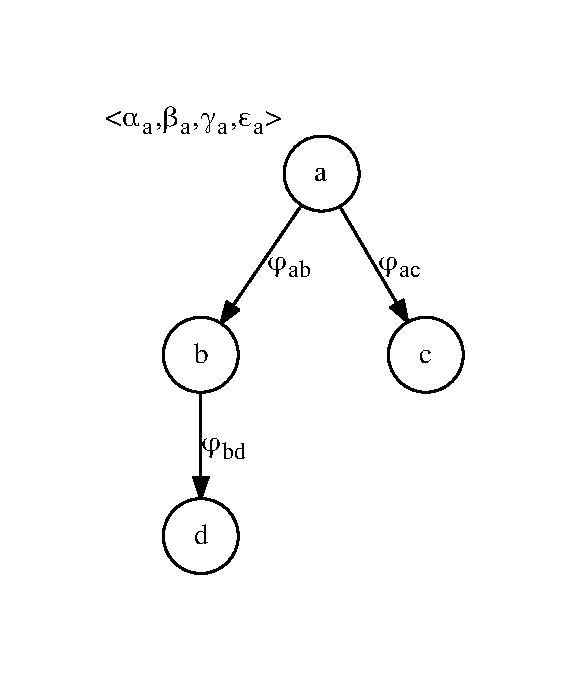
\includegraphics[width=.4\textwidth]{fig/base-graph.eps}
    }
  \end{center}
    \caption{A base question-and-item graph. Here, the $\alpha_a$ is the item
    discrimination for a, $\beta_a$ is the difficulty, $\gamma_a$ is the
    probability of guessing, and $\epsilon_a$ is the variance in the response
    set due to "error" (the student's composite score).}
 \end{wrapfigure}


 \begin{wrapfigure}{R}{.5\textwidth}
  \begin{center}
    \fbox{
      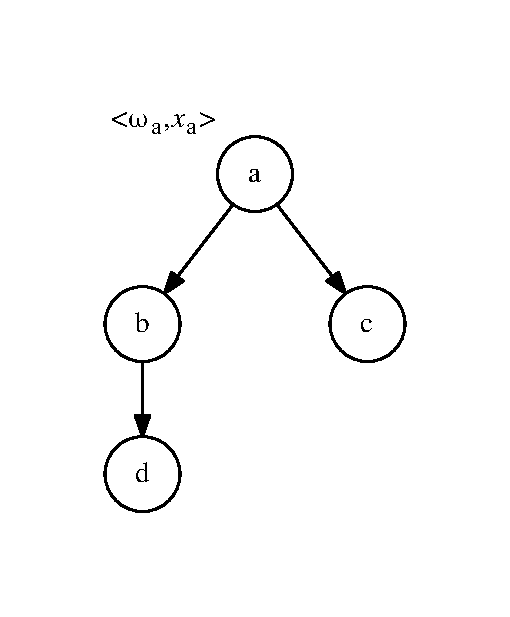
\includegraphics[width=.4\textwidth]{fig/student-graph.eps}
    }
    \caption{A student-specific graph. Here, the boolean $\omega_a$ indicates
    whether or not the student has answered question a, and $x_a$  is the
    score.  The graph has the same structure as the base graph.}
  \end{center}
 \end{wrapfigure}


 \begin{figure}
  \begin{tabular}{lcccccc}
                 & Knowledge & Comprension & Application & Analysis & Evaluation & Synthesis   \\
   Expressions   &   4       &      3      &      2      &    1     &      1     &      1      \\
   Boolean Logic &   3       &      1      &     .5      &   -1     &     -1.5   &     -2      \\
   If-Statements &   2       &     .5      &      0      &   -1.5   &     -2     &     -2.5    \\
   For-Loops     &   1       &      0      &     -1      &    -2    &     -3     &     -3      \\
  \end{tabular}

  \caption{An example trait abiilty table $\Theta_s$.  Rows are concepts and
  columns are Bloom levels. Here it is shown that the student performs well on
  expressions generally, and has sufficient knowledge of all topics.  The
  points of impasse exist in the analysis of boolean logic, application of
  if-statements and comprehension of for-loops.  Candidates for question
  selection include $\theta_{22}$ and $\theta_{31}$.}

 \end{figure}


 %\begin{figure}
  \begin{algorithm}
   \begin{algorithmic}[1]

     \Globals
       \State $\Theta$: trait ability matrix
     \EndGlobals

    \item[]
    \Function{node-properties}{$node$}
      \State \Return $(c, b, \alpha, \beta, \gamma, \epsilon)$.
    \EndFunction

    \item[]
    \Function{node-edges}{$node$}
      \State \Return $E$.
    \EndFunction

    \Function{select-category}{}
      \State $(i ,j) \gets argmin_{i, j}$ $| \Theta_{s} |$.
      \State \Call{question-search}{$C_i, B_j, root$}.
    \EndFunction

    \item[]
    \Function{question-search}{$c_t, b_t, node$}
      \State $(c, b, \alpha, \beta, \gamma, \epsilon) \gets \Call{node-properties}{node}$.
      \If{$b = b_t$ and $c == c_t$}
        \Return $node$.
      \EndIf
      \State $E \gets$ \Call{node-edges}{$node$}.
      \ForAll{$e \in E$}
         \State \Call{question-search}{$c_t, b_t, e$}.  
      \EndFor
    \EndFunction

   \end{algorithmic}
   \caption{\emph{Select Next Question}.}
  \end{algorithm}

  \begin{algorithm}
   \caption{\emph{Update Trait Table}.}
   \begin{algorithmic}

     \Globals
       \State $\Theta$: trait ability matrix
     \EndGlobals

     \item[]
     \Function{update-table}{r}
       \State $x \gets $ \Call{grade}{r}
     \EndFunction

   \end{algorithmic}
  \end{algorithm}


\section{Methodology}

\section{Analysis}


\end{document}
